% PROBLEM INTERPRETATION
Now we will interpret the uncertainty characterization subproblem A of the NASA Langley UQ challenge \cite{NASA:Crespo2014:Proc,NASA:Crespo2013:FAQ:URL} in Bayesian terms.
For that purpose we will compose an appropriate Bayesian multilevel model and formulate the main objective, i.e.\ the reduction of epistemic uncertainties, as Bayesian calibration of this multilevel model.
% UNCERTAINTY MODEL
Inputs \((p_1,p_2,p_3,p_4,p_5)\) of the forward model \(\mathcal{M} \equiv h_1\) are subject to uncertainty.
Model inputs \(\bm{\zeta} \equiv p_3\), that are subject to aleatory variability, constitute the category I parameters.
There is epistemic uncertainty about the true value of the category II model parameter \(\bm{m} \equiv p_2\).
Category III subsumes those parameters \(\bm{x} \equiv (p_1,p_4,p_5)\) that are subject to a mixed-type uncertainty.
% PRIOR MODELS
Generally, population distributions of experiment-specific variables are provided by the organizers of the challenge problem,
whereas prior marginals of the QoI are uninformative interpretations of the epistemic intervals given.

\subsection{Category I: Aleatory uncertainty}
For experiments \(i=1,\ldots,n\) category I model inputs \(\bm{\zeta} \equiv p_3 \in [0,1]\) take on experiment-specific realizations \(p_{3,i}\).
The population distribution is a uniform distribution \(\mathcal{U}(p_{3,i} \cond a_3,b_3)\) determined by perfectly known hyperparameters \(\bm{\theta}_{\bm{Z}} \equiv \bm{\theta}_3 = (a_3,b_3)\) with \((a_3,b_3) = (0,1)\).
We write this as follows
\begin{equation} \label{eq:JAIS:Distr:p3}
  (P_{3,i} \cond \bm{\theta}_3) \sim f_3(p_{3,i} \cond \bm{\theta}_3) = \mathcal{U}(p_{3,i} \cond 0,1).
\end{equation}
It corresponds to a prescribed aleatory variability or structural uncertainty that is irreducible in the sense that
by analyzing available data \(\perfect{y}_i\) for \(i=1,\ldots,n\) ``past'' realizations \(p_{3,i}\) could be inferred in principle,
whereas the knowledge about ``future'' realizations \(p_{3,\further{i}}\) with \(\further{i}>n\) cannot be improved.

\subsection{Category II: Epistemic uncertainty}
Category II model inputs are physically fixed yet unknown model parameters \(\bm{m} \equiv p_2 \in [0,1]\).
A given epistemic interval \(\Delta = [0,1]\) is known to contain the true value of \(p_2\) prior to any data analysis.
We translate this available information into a flat and uniform Bayesian prior probability density
\begin{equation} \label{eq:JAIS:Prior:p2}
  P_2 \sim \pi_2(p_2) = \mathcal{U}(p_2 \cond 0,1).
\end{equation}
It represents an a priori degree of plausibility of the true value \(p_2\) and it is reducible in the sense that Bayesian updating provides an a posteriori degree of evidence.
The quantification of parametric Bayesian priors is a controversial business.
Priors go beyond bare interval-like statements by assigning a relative probability structure over the set of admissible values.
Thus more generally any prior distribution with nonzero support over the priorly admissible set \(\Delta\) that vanishes elsewhere could be considered appropriate.

\subsection{Category III: Mixed uncertainty}
Category III comprises those model inputs \(\bm{x} \equiv (p_1,p_4,p_5)\) that are subject to aleatory variability across experiments \(i=1,\ldots,n\).
The natural variability is parametrized by hyperparameters \(\bm{\theta}_{\bm{X}} \equiv (\bm{\theta}_1,\bm{\theta}_{45})\) that are epistemically uncertain themselves.
This is a mixed-type uncertainty model that in less Bayesian contexts is sometimes referred to as imprecise probability or distributional p-box \cite{Uncertainty:Helton2004,Uncertainty:Helton2011}.

\subsubsection{Unimodal beta}
Model inputs \(p_1 \in [0,1]\) are distributed according to a unimodal beta distribution.
% PARAMETRIZATION
Beta distributions \(\mathrm{Beta}(p_{1,i} \cond \alpha_1,\beta_1)\) are commonly parametrized by shape hyperparameters \(\alpha_1,\beta_1 > 0\).
Instead we herein parametrize the beta distribution \(\mathrm{Beta}(p_{1,i} \cond \mu_1,\sigma^2_1)\) by its mean \(\mu_1\) and variance \(\sigma^2_1\).
Thus with unknown hyperparameters \(\bm{\theta}_1 \equiv (\mu_1,\sigma^2_1)\) experiment-specific realizations \(p_{1,i}\) are drawn from the population distribution
\begin{equation} \label{eq:JAIS:Distr:p1}
  (P_{1,i} \cond \bm{\theta}_1) \sim f_1(p_{1,i} \cond \bm{\theta}_1)  = \mathrm{Beta}(p_{1,i} \cond \mu_1,\sigma^2_1).
\end{equation}
% PROPERTIES
To begin with, given the shape parameters \((\alpha_1,\beta_1)\), the expected value \(\mu_1 = \mathds{E}[p_1]\) and the variance \(\sigma^2_1 = \mathrm{Var}[p_1]\)
of the density function \(\mathrm{Beta}(p_{1,i} \cond \mu_1,\sigma^2_1)\) are given as
\begin{equation} \label{eq:JAIS:Beta:Transform2Stat}
  \mu_1 = \frac{\alpha_1}{\alpha_1 + \beta_1}, \quad
  \sigma^2_1 = \frac{\alpha_1 \beta_1}{(\alpha_1 + \beta_1)^2 (\alpha_1 + \beta_1 + 1)}.
\end{equation}
Conversely, given the statistical moments \((\mu_1,\sigma^2_1)\), the shape parameters \((\alpha_1,\beta_1)\) of the density function \(\mathrm{Beta}(p_{1,i} \cond \alpha_1,\beta_1)\) can be obtained by
\begin{equation} \label{eq:JAIS:Beta:Transform2Shape}
  \alpha_1 = \left( \frac{\sigma^2_1 + \mu_1^2-\mu_1}{\sigma^2_1} \right) \left( -\mu_1 \right), \quad
  \beta_1  = \left( \frac{\sigma^2_1 + \mu_1^2-\mu_1}{\sigma^2_1} \right) \left( \mu_1 - 1 \right).
\end{equation}
% EPISTEMIC INTERVALS
The required unimodality, i.e.\ the fact that the distribution features a single mode within its support, translates into \(\alpha_1,\beta_1 > 1\).
Moreover the problem setup requires \(\nicefrac{3}{5} \leq \mu_1 \leq \nicefrac{4}{5}\) and \(\nicefrac{1}{50} \leq \sigma^2_1 \leq \nicefrac{1}{25}\).
% BAYESIAN PRIOR
In order to adopt this epistemic uncertainty model for the hyperparameters \(\bm{\theta}_1\) we state the uniform hyperprior
\begin{equation} \label{eq:JAIS:Prior:Hyper:p1}
  \begin{aligned}
    \bm{\Theta}_1 &\sim \pi_1(\bm{\theta}_1) = \mathcal{U}(\bm{\theta}_1 \cond \mathcal{D}_{\bm{\theta}_1}), \;\, \text{with} \\
    \mathcal{D}_{\bm{\theta}_1}
    &= \big\{ (\mu_1,\sigma^2_1) \in \mathds{R}^2 \cond \nicefrac{3}{5} \leq \mu_1 \leq \nicefrac{4}{5}, \, \nicefrac{1}{50} \leq \sigma^2_1 \leq \nicefrac{1}{25}, \, \alpha_1>1, \, \beta_1>1 \big\}.
  \end{aligned}
\end{equation}
If \(\lambda(\mathcal{D}_{\bm{\theta}_1})\) is the volume of the set \(\mathcal{D}_{\bm{\theta}_1} \subset \mathds{R}^2\),
then the uniform density \cref{eq:JAIS:Prior:Hyper:p1} is \(1/\lambda(\mathcal{D}_{\bm{\theta}_1})\) on \(\mathcal{D}_{\bm{\theta}_1}\) and zero elsewhere.
% NORMALIZATION CONSTANT
In practice the normalization constant \(\lambda(\mathcal{D}_{\bm{\theta}_1})\) is unknown, but since priors are flat and only ratios are compared in the MH correction \cref{eq:JAIS:MCMC:MHCorrection}, 
only the set membership of MCMC proposals has to be determined.
\par % PRACTICALLY SPEAKING
Consequently we can treat the prior \cref{eq:JAIS:Prior:Hyper:p1} as \(\pi_1(\bm{\theta}_1) = \pi(\mu_1) \, \pi(\sigma^2_1)\) with independent marginals
\(\pi(\mu_1) = \mathcal{U}(\mu_1 \cond \nicefrac{3}{5},\nicefrac{4}{5})\) and \(\pi(\sigma^2_1) = \mathcal{U}(\sigma^2_1 \cond \nicefrac{1}{50},\nicefrac{1}{25})\)
and reject MCMC proposals that do not respect \(\alpha_1,\beta_1 > 1\) with the aid of \cref{eq:JAIS:Beta:Transform2Shape}.
% AMBIGUITY
This practical prior choice is ambiguous in the sense that priors could be assumed for shape parameters \((\alpha_1,\beta_1)\), too.
However, this could yield improper prior distributions.
From an engineering point of view, we consider \((\mu_1,\sigma^2_1)\) statistically more ``natural'' than the shape parameters.
In addition they underlie strong prior constraints which is advantageous to exploring the posterior by means of MCMC.

\subsubsection{Correlated Gaussian}
The model inputs \(p_4,p_5 \in \mathds{R}\) are modeled as possibly correlated Gaussian random variables.
Across the experiments \(i=1,\ldots,n\) these model inputs take on different unknown realizations \((p_{4,i},p_{5,i})\).
This inherently aleatory variability is represented by the population distribution
\begin{equation} \label{eq:JAIS:Distr:p45}
  \big( (P_{4,i},P_{5,i}) \cond \bm{\theta}_{45} \big) \sim f_{45} \big( (p_{4,i},p_{5,i}) \cond \bm{\theta}_{45} \big) = \mathcal{N} \big( (p_{4,i},p_{5,i}) \cond \bm{\mu}_{45},\bm{\Sigma}_{45} \big).
\end{equation}
% PARAMETRIZATION
For \(j=4,5\) the means \(\mu_j = \mathds{E}[p_j]\), variances \(\sigma_j^2 = \mathrm{Var}[p_j]\) and the coefficient of correlation
\(\rho_{45} = \mathds{E}[(p_4-\mu_4)(p_5-\mu_5)]\) constitute the hyperparameters \(\bm{\theta}_{45} \equiv (\mu_4,\sigma^2_4,\mu_5,\sigma^2_5,\rho_{45})\).
Those hyperparameters are unknown constants that determine the mean \(\bm{\mu}_{45}\) and the covariance matrix \(\bm{\Sigma}_{45}\) of the bivariate normal density by
\begin{equation}
  \bm{\mu}_{45} = \begin{pmatrix}
                    \mu_4 \\
                    \mu_5
                  \end{pmatrix},
  \quad
  \bm{\Sigma}_{45} = \begin{pmatrix}
                       \sigma_4^2 & \rho_{45} \, \sigma_4 \, \sigma_5 \\
                       \rho_{45} \, \sigma_4 \, \sigma_5 & \sigma_5^2
                     \end{pmatrix}.
\end{equation}
% PRIOR MODEL
Besides the natural bounds \(\lvert \rho_{45} \rvert \leq 1\) it is requested that \(-5 \leq \mu_j \leq 5\) and \(\nicefrac{1}{400} \leq \sigma_j^2 \leq 4\).
We translate these intervals into flat and independent marginals \(\pi(\mu_j)\), \(\pi(\sigma^2_j)\) and \(\pi(\rho_{45})\) of the common hyperprior \(\pi_{45}(\bm{\theta}_{45})\) by
\begin{equation} \label{eq:JAIS:Prior:Hyper:p45}
  \left.
  \begin{aligned}
    \pi(\mu_j)      &= \mathcal{U}(\mu_j \cond -5,5), \\
    \pi(\sigma^2_j) &= \mathcal{U}(\sigma^2_j \cond \nicefrac{1}{400},4), \\
    \pi(\rho_{45})  &= \mathcal{U}(\rho_{45} \cond -1,1),
  \end{aligned}
  \;\, \right\} \;\, \bm{\Theta}_{45} \sim \pi_{45}(\bm{\theta}_{45}) = \left( \prod\limits_{j=4}^5 \pi(\mu_j) \, \pi(\sigma^2_j) \right) \pi(\rho_{45}).
\end{equation}
% AMBIGUITY
Insofar as priors for spread hyperparameters could refer to standard deviations or variances alike,
the ambiguity in quantifying parametric Bayesian priors becomes especially obvious for these type of hyperparameters.

\subsection{Bayesian problem statement}
% PROBLEM STATEMENT
The primary objective of the NASA UQ challenge subproblem A is the reduction of epistemic uncertainties
of the true values of the forward model parameter \(p_2\) and the hyperparameters \((\bm{\theta}_1,\bm{\theta}_{45})\) \cite{NASA:Crespo2014:Proc}.
% MODEL INPUT UNCERTAINTY, GIVEN DATA, FORWARD MODEL
In order to accomplish that goal, the forward model, a set of data and prior knowledge is available.
% COMPUTATIONAL FORWARD MODEL
Preventing to reverse-engineer its mathematical character and numerical implementation, the forward model \(h_1\) is distributed as a protected MATLAB p-code file, i.e.\ a ``blackbox'' model.
% DATA MODEL
Available data \(\tuple{\perfect{y}_i}_{1 \leq i \leq 50}\) comprises \(n = 50\) scalar observations \(\perfect{y}_i = h_1(p_{1,i},p_2,p_{3,i},p_{4,i},p_{5,i})\)
which have been realized as forward model responses complying with the true uncertainty model of forward model inputs, i.e.\
the model parameter \(p_2\) takes on its true value and \((\tuple{p_{1,i}},\tuple{p_{3,i}},\tuple{p_{4,i}},\tuple{p_{5,i}})\) have been randomly sampled from their true population distributions.
% IMPERFECT DATA
Notwithstanding that the observations provided are ``perfect'', in general they might very well be subject to an additional model-measurement discrepancy, i.e.\ ``imperfect'' \cite{NASA:Crespo2013:FAQ:URL}.
% DATA CONFIGURATIONS
Data have been arranged into two distinct configurations of observations \(\tuple{\perfect{y}_i}_{1 \leq i \leq 25}\) and \(\tuple{\perfect{y}_i}_{26 \leq i \leq 50}\)
whose separate and joint analysis is envisaged to indicate how the number \(n\) of processed samples impacts the significance of the final results.
\par % PRIOR KNOWLEDGE
The available prior knowledge has been translated into parametric and structural Bayesian prior distributions.
We have pointed out that this formulation endows the problem with a subjectivist interpretation of probability
and suffers from the ambiguity in the chosen parametric prior and its influence on the resulting posterior.
% AMPLE SCOPE
The problem statement as well as the framework and the algorithms introduced so far grant ample scope
of formulating and solving the problem as Bayesian inference of the QoI \((p_2,\bm{\theta}_1,\bm{\theta}_{45})\) within a multilevel context.
% PERFECT DATA
In the first place the Bayesian multilevel model \cref{eq:JAIS:PerfectData:Model},
defined by parametric priors \cref{eq:JAIS:Prior:Hyper:p1,eq:JAIS:Prior:Hyper:p45,eq:JAIS:Prior:p2} and structural priors \cref{eq:JAIS:Distr:p3,eq:JAIS:Distr:p1,eq:JAIS:Distr:p45},
establishes the natural framework for solving the original problem posed.
For the sake of completeness the devised multilevel model is summarized as
\begin{equation}
  \begin{aligned}
    (\perfect{Y}_i \cond p_2,\bm{\theta}_1,\bm{\theta}_{45},\bm{\theta}_3) &\sim f(\perfect{y}_i \cond p_2,\bm{\theta}_1,\bm{\theta}_{45},\bm{\theta}_3), \\
    P_2 & \sim \pi_2(p_2) = \mathcal{U}(p_2 \cond 0,1), \\
    (P_{1,i} \cond \bm{\theta}_1) &\sim f_1(p_{1,i} \cond \bm{\theta}_1)  = \mathrm{Beta}(p_{1,i} \cond \mu_1,\sigma^2_1), \\
    \big( (P_{4,i},P_{5,i}) \cond \bm{\theta}_{45} \big) &\sim f_{45} \big( (p_{4,i},p_{5,i}) \cond \bm{\theta}_{45} \big) = \mathcal{N} \big( (p_{4,i},p_{5,i}) \cond \bm{\mu}_{45},\bm{\Sigma}_{45} \big), \\
    \bm{\Theta}_1 &\sim \pi_1(\bm{\theta}_1) = \mathcal{U}(\bm{\theta}_1 \cond \mathcal{D}_{\bm{\theta}_1}), \\
    \bm{\Theta}_{45} &\sim \pi_{45}(\bm{\theta}_{45}) =  \pi(\mu_4) \, \pi(\sigma^2_4) \, \pi(\mu_5) \, \pi(\sigma^2_5) \, \pi(\rho_{45}), \\
    (P_{3,i} \cond \bm{\theta}_3) &\sim f_3(p_{3,i} \cond \bm{\theta}_3) = \mathcal{U}(p_{3,i} \cond 0,1).
  \end{aligned}
\end{equation}
The corresponding posterior distribution \cref{eq:JAIS:PerfectData:Posterior} of the QoI \((p_2,\bm{\theta}_1,\bm{\theta}_{45})\)
follows Bayesian data analysis of the given forward model responses \(\tuple{\perfect{y}_i}\),
i.e.\ realizations of random variables \((\perfect{Y}_i \cond p_2,\bm{\theta}_1,\bm{\theta}_{45},\bm{\theta}_3)\).
\par % IMPERFECT DATA
In the second place one could solve the inverse problem posed in the presence of additional measurement noise.
To that end the Bayesian multilevel model \cref{eq:JAIS:Multilevel:Model} establishes the proper framework.
% PERTURBING
Synthetic and noisy observations \(y_i = \perfect{y}_i + \varepsilon_i\) could be obtained by perturbing the given model responses \(\perfect{y}_i\)
with residuals \(\varepsilon_i\) that are randomly sampled from prescribed distributions \(f_{E_i}(\varepsilon_i) = \mathcal{N}(\varepsilon_i \cond 0,\sigma^2_i)\).
Parameters of the residual model, i.e.\ the residual variances \(\sigma_i^2\), could either be treated as knowns or as further unknowns.
% POSTERIOR
By analyzing ``imperfect'' data \(\tuple{y_i}\), i.e.\ realizations of random variables \((Y_i \cond p_{1,i},p_2,p_{3,i},p_{4,i},p_{5,i})\),
and treating latent variables \((\tuple{p_{1,i}},\tuple{p_{3,i}},\tuple{p_{4,i}},\tuple{p_{5,i}})\) as nuisance,
inference of the QoI would be based on the posterior \cref{eq:JAIS:Multilevel:MarginalPosterior}.
% NASA DAG
A DAG of the Bayesian multilevel model corresponding to our challenge problem interpretation with ``perfect'' and ``imperfect'' data, respectively, is depicted in \cref{fig:JAIS:NASA:DAG}.
\begin{figure}[htbp]
  \centering
  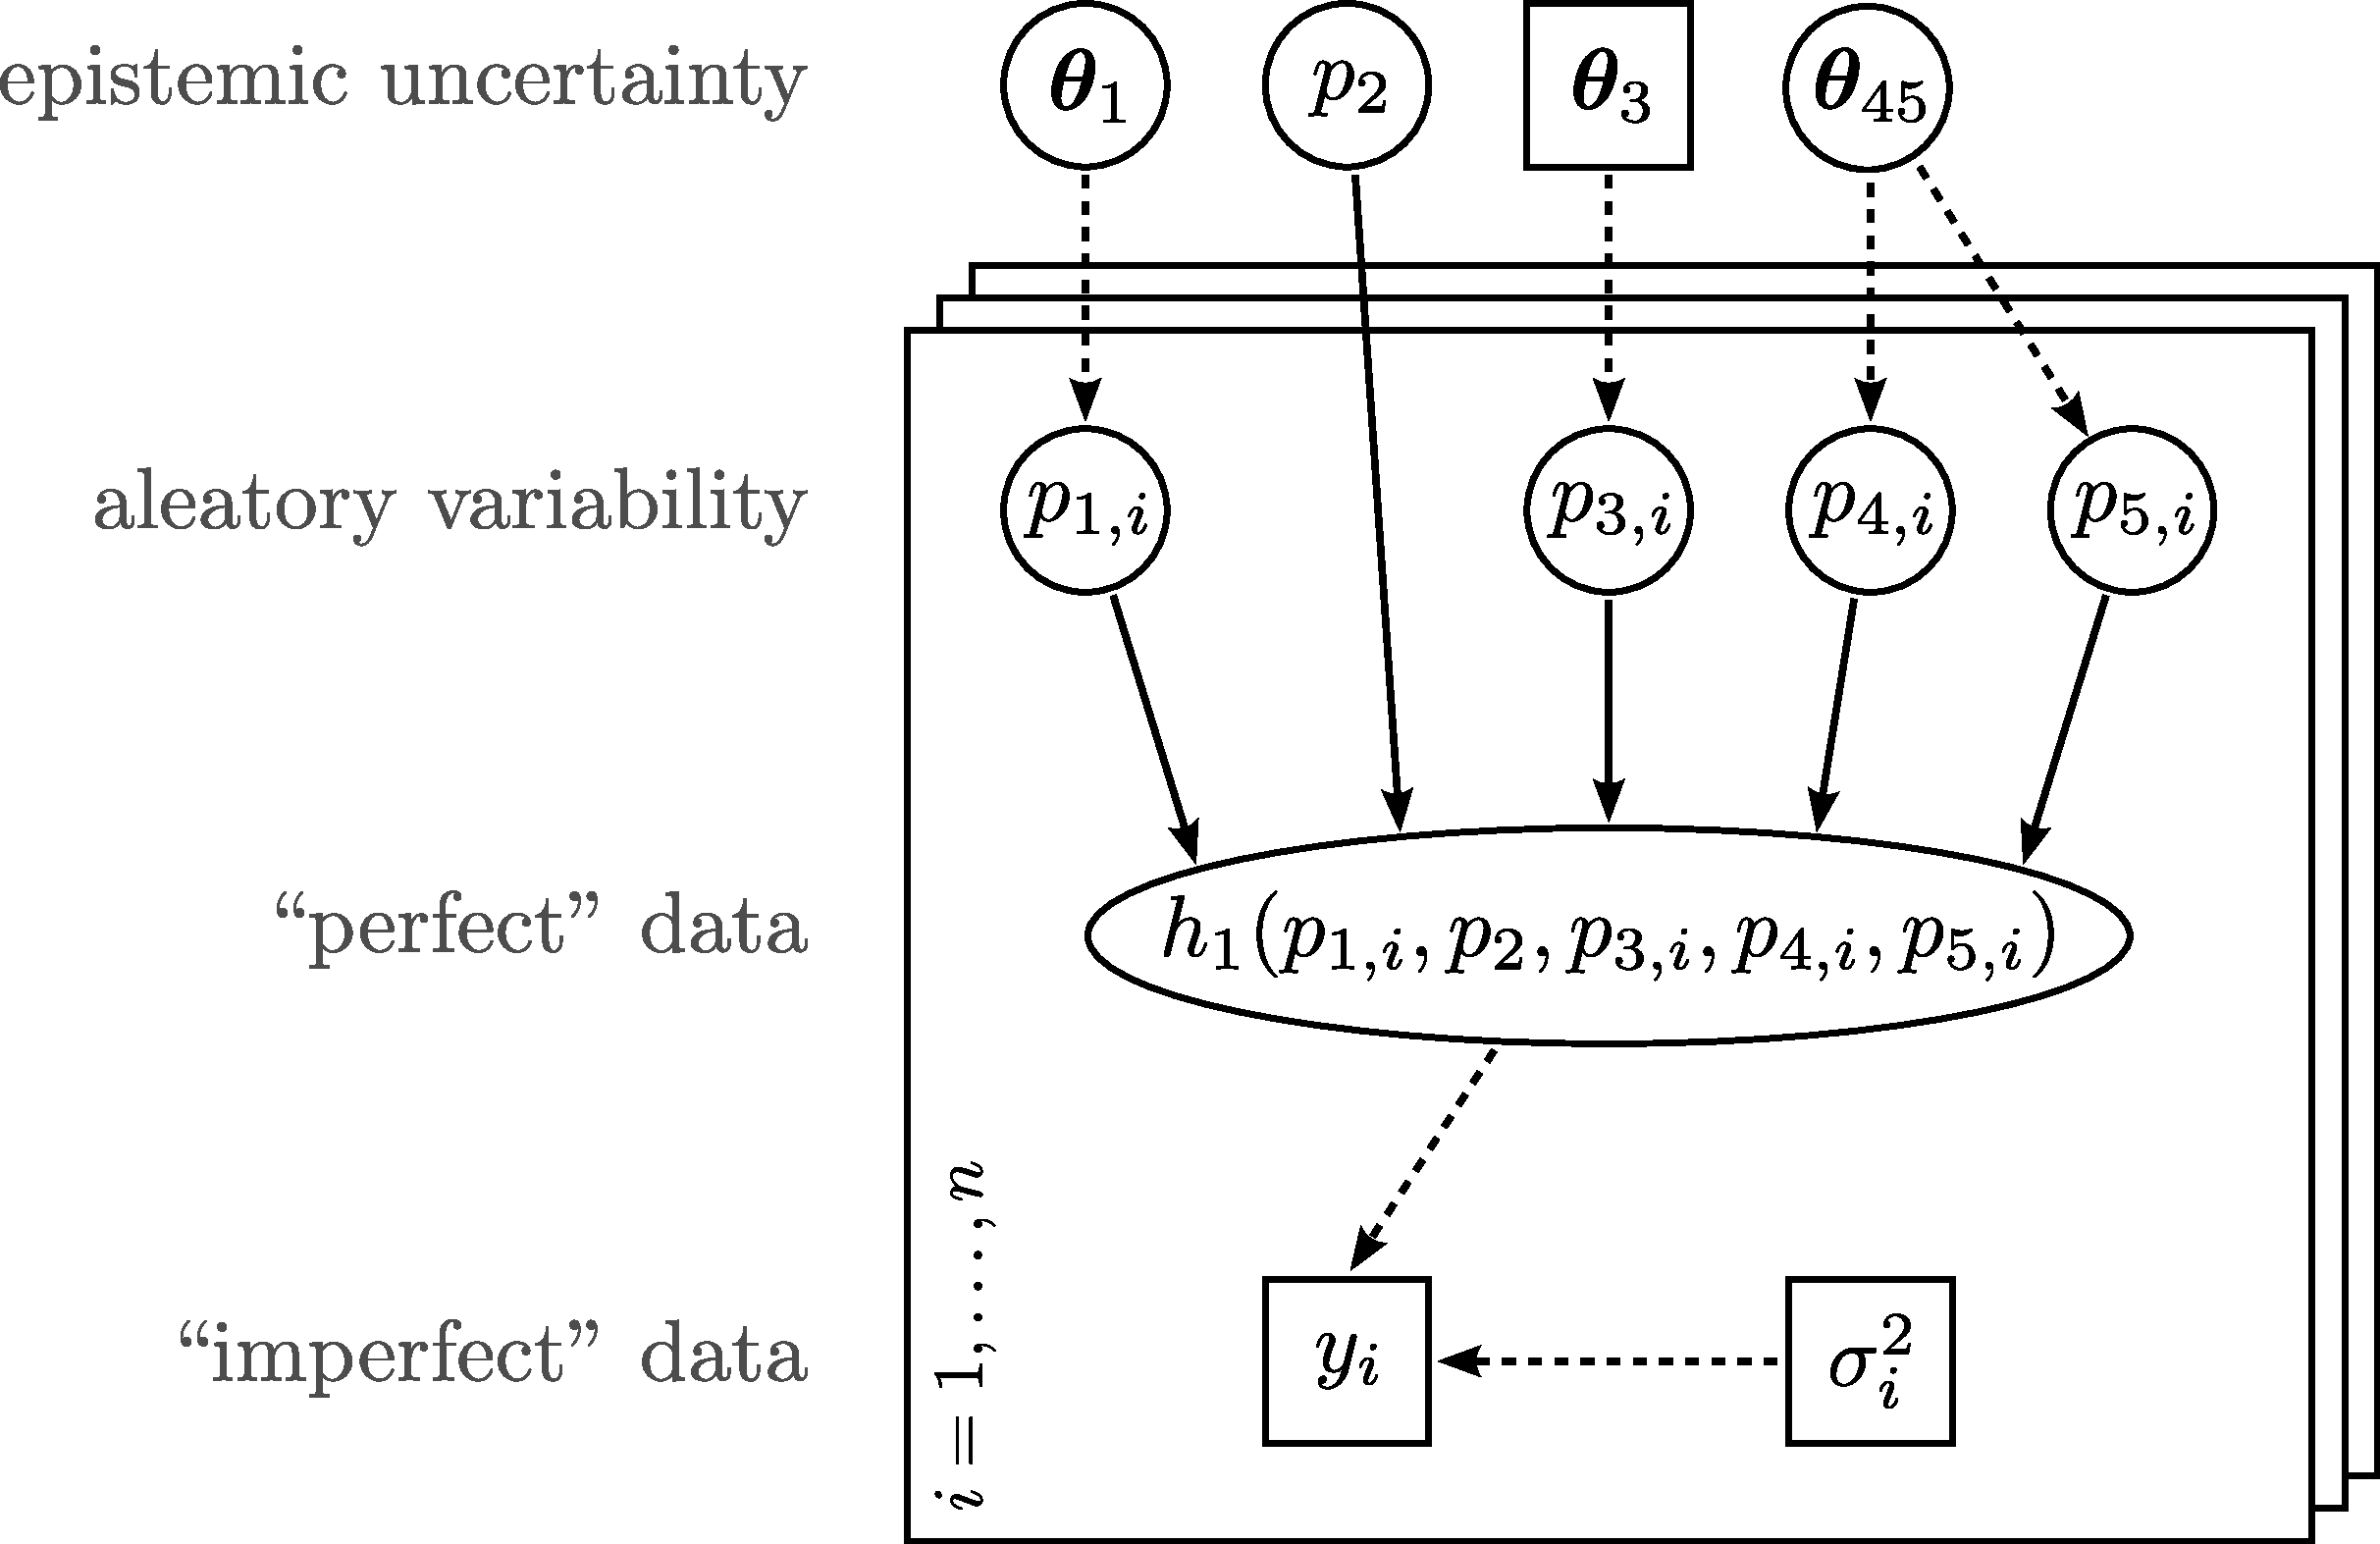
\includegraphics[height=\JAISdagHeight]{fig_JAIS_DAG_NASA}
  \caption[DAG of the NASA UQ challenge subproblem A]{DAG of the NASA UQ challenge subproblem A.
           The hyperparameters \(\bm{\theta}_1\) and \(\bm{\theta}_{45}\) and the forward model parameter \(p_2\) located at the ``highest'' hierarchical level are the QoI.
           Realizations \((\tuple{p_{1,i}},\tuple{p_{3,i}},\tuple{p_{4,i}},\tuple{p_{5,i}})\) on the ``intermediate'' problem level are considered nuisance.
           ``Perfect'' \(\perfect{y}_i = h_1(p_{1,i},p_2,p_{3,i},p_{4,i},p_{5,i})\) or ``imperfect'' data \(y_i = \perfect{y}_i + \varepsilon_i\) constitute the ``lowest'' model layer.
          }
  \label{fig:JAIS:NASA:DAG}
\end{figure}